\documentclass[11pt]{article}

% ---------- Packages ----------
\usepackage[utf8]{inputenc}
\usepackage[T1]{fontenc}
\usepackage[margin=1in]{geometry}
\usepackage{amsmath, amssymb}
\usepackage{booktabs}
\usepackage{array}
\usepackage{enumitem}
\usepackage{xcolor}
\usepackage{tikz}
\usetikzlibrary{shapes.geometric, arrows.meta, positioning, fit, backgrounds, calc}
\usepackage{listings}
\usepackage{hyperref}
\hypersetup{colorlinks=true, linkcolor=blue, urlcolor=blue}

% ---------- TikZ styles ----------
\tikzset{
  block/.style   = {rectangle, draw, rounded corners, align=center,
                     fill=blue!8, minimum height=1cm, minimum width=2.8cm,
                     inner sep=6pt},
  group/.style   = {rectangle, draw, dashed, rounded corners, inner sep=10pt},
  arrow/.style   = {-{Stealth[length=3mm]}, thick},
  biarrow/.style = {{Stealth[length=3mm]}-{Stealth[length=3mm]}, thick},
}

% ---------- Listings style ----------
\definecolor{codebg}{gray}{0.96}
\lstset{
  basicstyle=\ttfamily\small,
  backgroundcolor=\color{codebg},
  frame=single,
  rulecolor=\color{gray!40},
  breaklines=true,
  columns=fullflexible,
  keepspaces=true,
  showstringspaces=false,
  xleftmargin=6pt, xrightmargin=6pt,
  aboveskip=8pt, belowskip=8pt,
}

\title{\textbf{Phase 0 --- Understand My Computer}\\[4pt]
\large VLA Robot Project --- Environment Verification}
\author{Robotics + AI Mentor Notes}
\date{\today}

\begin{document}
\maketitle

\begin{abstract}
\noindent Goal of this phase: \textbf{verify} what is already installed. Install
nothing yet. First we understand the big picture, then we check the environment in
small batches.
\end{abstract}

\tableofcontents
\bigskip
\hrule

% =====================================================================
\section{The Complete VLA Robot Architecture (high-level)}

A VLA robot \textbf{turns pixels + words into motion}, then watches the result and
adjusts.

\begin{center}
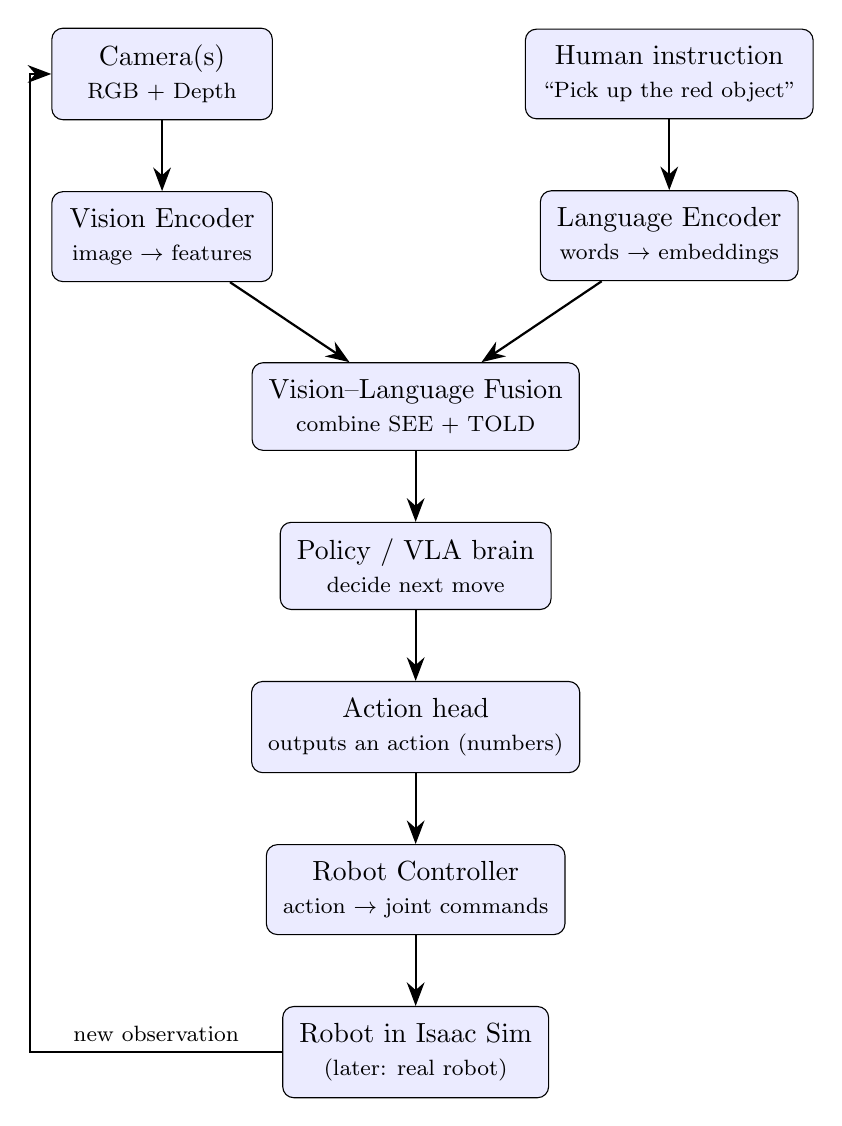
\begin{tikzpicture}[node distance=0.9cm and 1.4cm]
  \node[block] (a) {Camera(s)\\{\footnotesize RGB + Depth}};
  \node[block, below=of a] (b) {Vision Encoder\\{\footnotesize image $\to$ features}};
  \node[block, right=3.2cm of a] (t) {Human instruction\\{\footnotesize ``Pick up the red object''}};
  \node[block, below=of t] (c) {Language Encoder\\{\footnotesize words $\to$ embeddings}};
  \node[block, below=1.6cm of $(b)!0.5!(c)$] (d) {Vision--Language Fusion\\{\footnotesize combine SEE + TOLD}};
  \node[block, below=of d] (e) {Policy / VLA brain\\{\footnotesize decide next move}};
  \node[block, below=of e] (f) {Action head\\{\footnotesize outputs an action (numbers)}};
  \node[block, below=of f] (g) {Robot Controller\\{\footnotesize action $\to$ joint commands}};
  \node[block, below=of g] (h) {Robot in Isaac Sim\\{\footnotesize (later: real robot)}};

  \draw[arrow] (a) -- (b);
  \draw[arrow] (t) -- (c);
  \draw[arrow] (b) -- (d);
  \draw[arrow] (c) -- (d);
  \draw[arrow] (d) -- (e);
  \draw[arrow] (e) -- (f);
  \draw[arrow] (f) -- (g);
  \draw[arrow] (g) -- (h);
  % feedback loop: new observation returns to the camera
  \draw[arrow] (h.west) -- ++(-3.2,0) node[midway, above, font=\footnotesize]{new observation} |- (a.west);
\end{tikzpicture}
\end{center}

\textbf{Key idea:} every arrow is just data (numbers/tensors) flowing between
boxes. Nothing is magic --- each box is a transformation you will eventually
understand and build.

\subsection{What each box does (plain intuition)}

\begin{center}
\begin{tabular}{@{}p{3cm}p{6.5cm}p{3.5cm}@{}}
\toprule
\textbf{Box} & \textbf{Plain-language job} & \textbf{Human analogy} \\
\midrule
Vision Encoder   & Compress an image into a compact list of numbers describing ``what's here'' & Eyes + visual cortex \\
Language Encoder & Turn the sentence into numbers a computer can reason with & Ears + language comprehension \\
Fusion           & Line up ``red thing at top-left'' with the word ``red'' & Brain connecting sight to speech \\
Policy (VLA)     & Decide the next move given scene + goal & Decision-making \\
Action head      & Produce concrete numbers: move hand +2\,cm right, close gripper & Motor planning \\
Controller       & Translate intent into actual joint motions & Spinal cord / muscles \\
Feedback loop    & Look again, check progress, correct & Hand--eye coordination \\
\bottomrule
\end{tabular}
\end{center}

\subsection{Two crucial teaching points}

\begin{enumerate}[leftmargin=*]
  \item \textbf{VLM vs VLA.} A \textbf{VLM} (Vision-Language Model) only
  \emph{describes} --- ``there is a red cube on the table.'' A \textbf{VLA}
  (Vision-Language-Action model) must \emph{act} --- output numbers that move a
  robot. That extra ``Action'' is the hard, robotics-specific part.
  (Deep dive in Phase~9.)
  \item \textbf{Classical first, then learned.} We build the \emph{classical}
  pipeline first (Phase~7) using hand-written computer vision + inverse
  kinematics, \textbf{before} replacing pieces with neural networks. You must
  understand what the VLA is \emph{replacing} to understand what it does.
\end{enumerate}

% =====================================================================
\section{Environment Checklist}

We only \textbf{verify} today --- \textbf{install nothing.}

\subsection{Hardware}
\begin{itemize}[leftmargin=*, label=$\square$]
  \item \textbf{NVIDIA GPU} (RTX class; Isaac Sim needs RTX ray tracing).
  Ideally $\geq 8$\,GB VRAM, better $\geq 12$\,GB for training.
  \item Decent CPU + $\geq 32$\,GB RAM recommended (16\,GB workable early).
  \item ${\sim}50+$\,GB free disk (Isaac Sim + datasets grow fast).
\end{itemize}

\subsection{Core software}
\begin{itemize}[leftmargin=*, label=$\square$]
  \item \textbf{Ubuntu 24.04} (target for ROS~2 Jazzy).
  \item \textbf{NVIDIA driver} (recent; supports your GPU + CUDA).
  \item \textbf{CUDA} (for PyTorch training later).
  \item \textbf{Python 3.12} (ships with Ubuntu 24.04 / ROS~2 Jazzy).
  \item \textbf{ROS~2 Jazzy} (believed installed --- we verify).
  \item \textbf{Git}.
\end{itemize}

\subsection{Simulation + AI (later phases --- just check presence today)}
\begin{itemize}[leftmargin=*, label=$\square$]
  \item \textbf{NVIDIA Isaac Sim} (4.x).
  \item \textbf{Isaac Lab} (optional; RL/learning workflows).
  \item \textbf{Gazebo} (optional alternative simulator).
  \item \textbf{GitHub CLI} (\texttt{gh}) --- optional convenience.
  \item \textbf{VS Code + GitHub Copilot} (already available).
\end{itemize}

% =====================================================================
\section{Verification Commands}

Run in a normal terminal (\texttt{Ctrl+Alt+T}). Paste back the full output of each.

\subsection{Batch 1 --- Foundation}

\paragraph{1. Ubuntu version}
\begin{lstlisting}[language=bash]
lsb_release -a
\end{lstlisting}
\begin{itemize}[leftmargin=*]
  \item \textbf{Does:} prints Linux distribution and version.
  \item \textbf{Expect:} \texttt{Description: Ubuntu 24.04.x LTS}.
  \item \textbf{If different:} 22.04 is fine to know; Jazzy prefers 24.04. Change
  nothing yet.
\end{itemize}

\paragraph{2. NVIDIA GPU + driver + driver-reported CUDA}
\begin{lstlisting}[language=bash]
nvidia-smi
\end{lstlisting}
\begin{itemize}[leftmargin=*]
  \item \textbf{Does:} shows GPU model, driver version, and max CUDA the driver
  supports.
  \item \textbf{Expect:} a table with \texttt{NVIDIA GeForce RTX ...},
  \texttt{Driver Version: 5xx.xx}, and \texttt{CUDA Version: 12.x} (top-right).
  \item \textbf{If ``command not found''/error:} driver not installed/loaded.
  Report the exact message; we diagnose, not blindly reinstall.
\end{itemize}

\paragraph{3. CUDA toolkit (compiler) --- separate from the driver}
\begin{lstlisting}[language=bash]
nvcc --version
\end{lstlisting}
\begin{itemize}[leftmargin=*]
  \item \textbf{Does:} checks if the CUDA \emph{toolkit} (dev tools) is installed
  (different from the driver's runtime).
  \item \textbf{Expect:} \texttt{release 12.x}.
  \item \textbf{If ``command not found'':} OK and common --- PyTorch ships its own
  CUDA runtime. Just report it.
\end{itemize}

\paragraph{4. Python}
\begin{lstlisting}[language=bash]
python3 --version
\end{lstlisting}
\begin{itemize}[leftmargin=*]
  \item \textbf{Does:} shows the system Python version.
  \item \textbf{Expect:} \texttt{Python 3.12.x} on Ubuntu 24.04.
  \item \textbf{If different:} note it; Jazzy is built against 3.12.
\end{itemize}

\subsection{Batch 2 --- (given after Batch 1 results)}
ROS~2 Jazzy, Git, GitHub CLI, Isaac Sim, Isaac Lab, Gazebo.

% =====================================================================
\section*{Next step}
\addcontentsline{toc}{section}{Next step}
Run \textbf{Batch 1} (4 commands) and paste the full output of each. Then I provide
Batch 2 and tell you exactly what --- if anything --- is missing.

\end{document}
